\documentclass{article}
\usepackage{amssymb,amsmath,chngcntr,graphicx,float,biblatex,tikz}

\begin{document}
\author{Timothy Smith}
\title{Griffiths}
\maketitle

\counterwithin*{equation}{section}
\section*{Problem 2.38}
A metal sphere of radius R, carrying charge q, is surrounded by a thick concentric metal shell( inner radius a , outer radius b).  The shell carries no net charge .
\\
\\
a) find the surface charge density $\sigma$ at R, at a, and  at b.
\\
\\
b) find the potential at the center, using infinity as the reference point.
\\
\\
c) Now the outer surface is touched to a ground wire, which drains of charge and lowers its potential to zero.  How do the answers to a) and b) change?
\\
\begin{center}
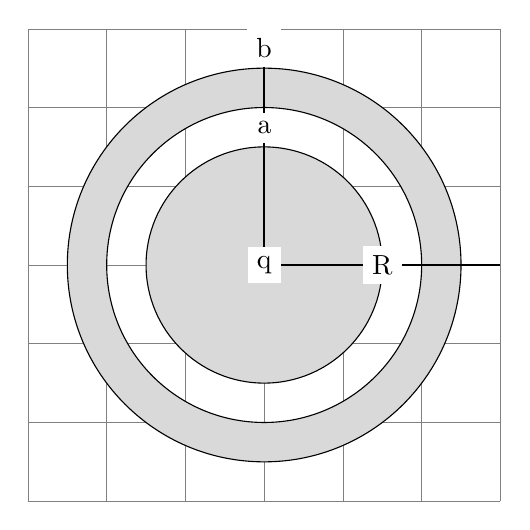
\begin{tikzpicture}
\draw[step=1cm,gray,very thin] (-2,-2) grid (4,4);
\draw[fill=gray!30,even odd rule]  (1,1) circle (2.5cm) (1,1) circle (2cm) (1,1) circle (1.5cm);
\draw [thick] (1,1) -- (4,1) node [pos=.5, fill=white] {R} node[pos=0, fill=white]{q};
\draw [thick] (1,1) -- (1,4)node[pos=.92, fill=white]{b} node[pos=0.58, fill=white]{a}node[pos=0, fill=white]{q} ;
\end{tikzpicture}
\end{center}

a) Since the charge at the center is positive, the surface charge densities are as follows.
\begin{align}
\sigma_R=\frac{q}{4{\pi}R^2}\\
\sigma_a=\frac{-q}{4{\pi}a^2}\\
\sigma_b=\frac{q}{4{\pi}b^2}
\end{align}
\\
b) To find our potential at the center, by using infinity as a reference point we create an integral for potential with those bounds.
\begin{equation}
V(r)
=
-\int_{\infty}^{0}\frac{1}{4{\pi}{\epsilon_0}}\frac{q}{r^2} dr
\end{equation}
This integral needs to account for the changes in charge throughout the respective areas thus the equation above becomes
\begin{equation}
V(r)
=
-\int_{R}^{0}\frac{1}{4{\pi}{\epsilon_0}}\frac{q}{r^2} dr-\int_{a}^{R}\frac{1}{4{\pi}{\epsilon_0}}\frac{q}{r^2} dr
-\int_{b}^{a}\frac{1}{4{\pi}{\epsilon_0}}\frac{q}{r^2} dr -\int_{\infty}^{b}\frac{1}{4{\pi}{\epsilon_0}}\frac{q}{r^2} dr
\end{equation}
Which results in
\begin{equation}
V(r)
=
\frac{1}{4{\pi}{\epsilon_0}}(\frac{q}{R}-\frac{q}{a}+\frac{q}{b})
\end{equation}
c) If the charge on the outer shell at b is drained so that the potential is zero. we can eliminate $\frac{q}{b}$ from equation 6. Also, equation 5 would change as we don't have to account for the charge density on b anymore. Thus our answer is 
\begin{equation}
V(r)
=
\frac{1}{4{\pi}{\epsilon_0}}(\frac{q}{R}-\frac{q}{a})
\end{equation}













\end{document}
